\chapter{Isotropic Propagation of Electromagnetic Waves}

\section{Maxwell's Equations in Vacuum}

As in vacuum charge density $\rho$ and current density $\vec{j}$ vanishes, So Maxwell's equations become:

\begin{enumerate}

   \item Gauss’s Law For Electricity

      \begin{equation}\label{gauss_law}
      \vec{\nabla}.\vec{E} = 0
      \end{equation}

   \item Gauss’s Law For Magnetism

      \begin{equation}
      \vec{\nabla}.\vec{B} = 0
      \end{equation}

   \item Faraday’s Law Of Induction

      \begin{equation}\label{faraday_induction}
      \vec{\nabla}\times\vec{E} = - \frac{\partial\vec{B}}{\partial t}
      \end{equation}

   \item Ampere’s Law

      \begin{equation}\label{amperes_law}
      \vec{\nabla}\times\vec{B} = \mu_{o}\epsilon_{o}\frac{\partial\vec{E}}{\partial t}
      \end{equation}

\end{enumerate}

Now if we apply curl to \eqref{faraday_induction}
%
   \begin{equation}\label{curl_of_induction}
   \vec{\nabla}\times(\vec{\nabla}\times\vec{E}) = - \vec{\nabla}\times(\frac{\partial\vec{B}}{\partial t})
   \end{equation}
%
using the definition of second derivative:
%
   \begin{equation}
   \vec{\nabla}\times(\vec{\nabla}\times\vec{A}) = \vec{\nabla}(\vec{\nabla}.\vec{A})-{\nabla}^2A
   \end{equation}
%
\eqref{curl_of_induction} becomes
%
   \begin{equation}
   \vec{\nabla}(\vec{\nabla}.\vec{E})-{\nabla}^2E = - \frac{\partial}{\partial t}(\vec{\nabla}\times\vec{B})
   \end{equation}

Substituting in \eqref{gauss_law} and \eqref{amperes_law} we get:
%
   \begin{equation}
   \nabla^2\vec{E} =  \mu_{o}\epsilon_{o}\frac{\partial^2\vec{E}}{\partial t^2}
   \end{equation}

Here each component of $\vec{E}$ satisfies the Electromagnetic Wave (EMW) Equation for electric field.

Similarly by applying curl to \eqref{amperes_law} we get the EMW equation for magnetic field:
%
   \begin{equation}
   \nabla^2\vec{B} =  \mu_{o}\epsilon_{o}\frac{\partial^2\vec{B}}{\partial t^2}
   \end{equation}
%
where $\mu_{o} = 1.257\times10^{-6} \, m kg s^{-2} A^{-2}$ and $\epsilon_{o} = 8.854 \times 10^{-12} m^{-3} kg^{-1} s^4 A^2$.

So that
%
   \begin{equation}
   \frac{1}{\sqrt{\mu_{o}\epsilon_{o}}} = 3\times10^8 \, ms^{-1}
   \end{equation}
%
which is equal to speed of light, $c$.

This means that electromagnetic waves travel through vacuum with the speed of light. Therefore light is an electromagnetic wave in nature, where electric field $\vec{E}$ and magnetic field $\vec{B}$ are perpendicular to each other and also to the direction of propagation of light.


\subsection{Poynting Vector}

The Poynting vector $\vec{S}$ represents the directional energy flux i.e, the energy transfer per unit area per unit time of an electromagnetic field.
%
   \begin{equation}
   \vec{S} = \frac{1}{\mu_{o}}(\vec{E}\times\vec{B})
   \end{equation}
%
which shows that the direction of power flow (propagation of EMW) at any point is normal to both $\vec{E}$ and $\vec{B}$. This implies that EMW/light is a Transverse wave. The SI unit of the Poynting vector is the watt per square meter, $W/m^{-2}$.


\section{Wave Solution In Spherical Coordinates}

Since an isotropic antenna radiates energy in a radially symmetric fashion the logical choice of coordinates for studying them is the spherical coordinate system.

\subsection{Spherical Coordinate System}

The vector derivatives in spherical coordinates are:

\begin{itemize}

   \item Gradient

      \begin{equation}
      \vec{\nabla} A = \frac{\partial A}{\partial r}\hat{r}+\frac{1}{r}\frac{\partial A}{\partial \theta}\hat{\theta}+\frac{1}{r\sin\theta}\frac{\partial A}{\partial \phi}\hat{\phi}
      \end{equation}

   \item Divergence

      \begin{equation}
      \vec{\nabla}.\vec{A} = \frac{1}{r^2}\frac{\partial}{\partial r}(r^2A_r)+\frac{1}{r\sin\theta}\frac{\partial}{\partial\theta}(\sin\theta A_\theta)+\frac{1}{r\sin\theta}\frac{\partial A_\phi}{\partial\phi}
      \end{equation}

   \item Curl

      \begin{equation}
      \vec{\nabla}\times\vec{A} = \frac{1}{r\sin\theta}\left[\frac{\partial}{\partial\theta}(\sin\theta A_\phi)-\frac{\partial A_\theta}{\partial\phi}\right]\hat{r}+\frac{1}{r}\left[\frac{1}{\sin\theta}\frac{\partial A_r}{\partial\phi}-\frac{\partial}{\partial r}(rA_\phi)\right]\hat{\theta}+\frac{1}{r}\left[\frac{\partial}{\partial r}(rA_\theta)-\frac{\partial A_r}{\partial \theta}\right]\hat{\phi}
      \end{equation}

   \item Laplacian

      \begin{equation}\label{laplacian}
      \nabla^2 \vec{A} = \frac{1}{r^2}\frac{\partial}{\partial r}(r^2\frac{\partial\vec{A}}{\partial r})+\frac{1}{r^2\sin\theta}\frac{\partial}{\partial\theta}(\sin\theta\frac{\partial\vec{A}}{\partial \theta})+\frac{1}{r^2\sin^2\theta}\frac{\partial^2\vec{A}}{\partial \phi^2}
      \end{equation}

\end{itemize}

\subsection{Deriving the Solution}

Starting from wave equation,

   \begin{equation}\label{wave_eq}
   \vec{\nabla}^2\vec{E}(\vec{s},t) =  \frac{1}{c^2}\frac{\partial^2\vec{E}(\vec{s},t)}{\partial t^2}
   \end{equation}
%
where
%
$\vec{E}(\vec{s},t) = \vec{E}(r,\theta,\phi,t)$
and using the definition of the Laplacian from \eqref{laplacian}, \eqref{wave_eq} becomes
%
   \begin{equation}
   \frac{1}{r^2}\frac{\partial}{\partial r}(r^2\frac{\partial\vec{E}(r,\theta,\phi,t) }{\partial r})+\frac{1}{r^2\sin\theta}\frac{\partial}{\partial\theta}(\sin\theta\frac{\partial \vec{E}(r,\theta,\phi,t)}{\partial \theta})+\frac{1}{r^2\sin^2\theta}\frac{\partial^2\vec{E}(r,\theta,\phi,t)}{\partial \phi^2} = \frac{1}{c^2}\frac{\partial^2\vec{E}(r,\theta,\phi,t)}{\partial t^2}
   \end{equation}

   For spherical symmetry, the solution is radial which means it cannot depend upon $\theta$ and $\phi$, so that
%
   \begin{equation}
   \frac{1}{r^2}\frac{\partial}{\partial r}(r^2\frac{\partial\vec{E}(\vec{r},t) }{\partial r})+\frac{1}{r^2\sin\theta}\frac{\partial}{\partial\theta}(\sin\theta\frac{\partial \vec{E}(\vec{r},t)}{\partial \theta})+\frac{1}{r^2\sin^2\theta}\frac{\partial^2\vec{E}(\vec{r},t)}{\partial \phi^2} = \frac{1}{c^2}\frac{\partial^2\vec{E}(\vec{r},t)}{\partial t^2}
   \end{equation}
%
where $\displaystyle \frac{\partial^2\vec{E}(\vec{r},t)}{\partial \theta^2}$ and $\displaystyle \frac{\partial^2\vec{E}(\vec{r},t)}{\partial \phi^2}$ become zero and we are left with
%
   \begin{equation}\label{wave_eqn_1}
   \begin{aligned}
      \frac{1}{r^2}\frac{\partial}{\partial r}(r^2\frac{\partial\vec{E}(\vec{r},t) }{\partial r}) = \frac{1}{c^2}\frac{\partial^2\vec{E}(\vec{r},t)}{\partial t^2}\\[0.5\baselineskip]
      \implies \frac{1}{r^2}[r^2\frac{\partial^2\vec{E}(\vec{r},t)}{\partial r^2}+\frac{\partial\vec{E}(\vec{r},t) }{\partial r}.(2r)] = \frac{1}{c^2}\frac{\partial^2\vec{E}(\vec{r},t)}{\partial t^2}
   \end{aligned}
   \end{equation}

   The LHS can be shown to be equal to $\frac{1}{r}\frac{\partial^2}{\partial r^2}[r\vec{E}(\vec{r},t)]$ so \eqref{wave_eqn_1} becomes
%
   \begin{equation}
   \frac{1}{r}\frac{\partial^2}{\partial r^2}[r\vec{E}(\vec{r},t)] = \frac{1}{c^2}\frac{\partial^2\vec{E}(\vec{r},t)}{\partial t^2} 
   \end{equation}
%
and multiplying by $r$
%
   \begin{equation}\label{wave_eqn_2}
   \frac{\partial^2}{\partial r^2}[r\vec{E}(\vec{r},t)] = \frac{1}{c^2}\frac{\partial^2}{\partial t^2}[r\vec{E}(\vec{r},t)]
   \end{equation}
%
where we have moved the $r$ inside on the RHS because the partial derivative is with respect to $t$ and not $r$.

If we now define $r\vec{E}(\vec{r},t) = \vec{T}(\vec{r},t)$ then \eqref{wave_eqn_2} becomes
%
   \begin{equation}
   \frac{\partial^2}{\partial r^2}[\vec{T}(\vec{r},t)] = \frac{1}{c^2}\frac{\partial^2}{\partial t^2}[\vec{T}(\vec{r},t)]
   \end{equation}

This is the wave equation in one dimension, with the well-known solution
%
\begin{equation}
\vec{T}(\vec{r},t) = \exp{i(kr-wt)}\hat{r}
\end{equation}
%
or equivalently
%
\begin{equation}
   \vec{T}(\vec{r},t) = \sin(kr-wt) \hat{r}
\end{equation}

As $r \vec{E}(\vec{r},t) = \vec{T}(\vec{r},t)$ so
%
   \begin{equation}
      r\vec{E}(\vec{r},t) = \sin(kr-wt) \hat{r}
   \end{equation}

And the final solution of wave equation is
%
\begin{equation}
   \vec{E}(\vec{r},t) = \frac{1}{r}\sin(kr-wt) \hat{r}
\end{equation}



\section{Calculating the Charge Density}

Charge density $\rho$ is a measure of electric charge per unit volume of space, in one, two or three dimensions.\\
More specifically, We have;\\
1. Linear charge density: is the amount of electric charge per unit length.\\
2. Surface charge density: is the amount of electric charge per surface area.\\
3. Volume charge density: is the amount of electric charge per volume.\\
From Gauss's law for electricity;\\
\begin{equation}
\vec{\nabla}.\vec{E} = \frac{\rho}{\epsilon_{o}}
\end{equation}
Charge density $\rho$ is\\
\begin{equation}
\rho = {\epsilon_{o}}(\vec{\nabla}.\vec{E})
\end{equation}
Now by using the equation for divergence, Eq. 1.13 and for $\vec{E}$, Eq. 1.28;\\
\begin{equation}
\rho = {\epsilon_{o}}[\frac{1}{r^2}\frac{\partial}{\partial r}(r^2\frac{1}{r}\sin(kr-wt))]
\end{equation}
\begin{equation}
\rho = {\epsilon_{o}}[\frac{1}{r^2}\frac{\partial}{\partial r}(r\sin(kr-wt))]
\end{equation}
\begin{equation}
\rho = {\epsilon_{o}}[\frac{1}{r^2}(r\cos(kr-wt).k+\sin(kr-wt))]
\end{equation}
Final equation for charge density is;\\
\begin{equation}
\rho = {\epsilon_{o}}[\frac{k}{r}\cos(kr-wt)+\frac{1}{r^2}\sin(kr-wt)]
\end{equation}
Which is not equal to zero, but it should be as we considered the case for vacuum; where there are no any charges and no charge density accordingly.\\

\subsection{Problem}
As determined solution Eq. 1.28, for wave equation in vacuum Eq. 1.16, is mathematically true and have no issue, But;\\
Why we did not get zero charge density?

\subsection{Solution}
The wave solution;\\
\begin{equation}
\vec{E}(\vec{r},t) = \frac{1}{r}\sin(kr-wt)
\end{equation}
is invalid for EMWs but is valid for acoustic/sound waves.\\

\subsubsection{Reason}
From Eq. 1.11, EMWs are transverse waves, but sound waves are longitudinal waves.\\
As we had spherically symmetric EMWs over a central point;
Carrying equal energy in all directions means isotropic EMWs.\\
And if we consider a sphere about the central point, at a large radius, then at that radius the wave over a reasonable area is essentially planar. We know electric and magnetic field of a plane wave in free space is always perpendicular to the direction of propagation of wave.\\
So, The electric field would have to be tangent to the surface of sphere everywhere, and continuous along that surface; Which means we have a continuous vector field, tangent to the surface of a sphere.\\
Now???\\
According to Hairy Ball Theorem
\begin{center}
	"For a sphere, If f is a continuous function that assigns a vector in $R^3$ to every point p on the sphere such that f(p) is always tangent to the sphere at point p then there is at least one point p such that f(p)=0."\\
\end{center}
This means that a continuous vector field, tangent to the surface of a sphere must fall to zero at one or more points on the sphere.\\
Which is inconsistent with the assumption of an isotropic EMWs.

\subsection{Isotropic Antenna}
As spherically isotropic EMWs are not possible, so there are no real isotropic radiators for EMWs, and because of this an isotropic electromagnetic antenna is a hypothetical antenna which does not exist in actual.\\
But, isotropic sound waves are possible as they are longitudinal waves and does not have any perpendicular component.

\section{Computational Work}
Our task is to construct the plot between distance and intensity, for multiple antenna sources arrange in a linear array and by managing phase between them we get a directive beam with maximum intensity .\\
First, we have to figure out an equation for intensity.\\
Let, we have a single source which is at distance L from the point of observation x=0, Now find the intensity at any point, say x from x=0, which is at distance r from the source?\\
As intensity is defined as power transferred per unit area, where the area is measured on the plane perpendicular to the direction of propagation of the energy. which is same as poynting vector, So by using the Eq. 1.11 for finding intensity.\\
\begin{equation}
I = \frac{1}{\mu_{o}}(\vec{E}\times\vec{B})
\end{equation}
Where $\vec{B} = \vec{E}/c$,\\
\begin{equation}
I = \frac{\sqrt{\mu_{o}{\epsilon_{o}}}}{\mu_{o}}E^2
\end{equation}
\begin{equation}
I = c\epsilon_{o}E^2
\end{equation}
So,\\
Intensity is directly proportional to square of electric field, i.e\\
\begin{equation}
I \propto E^2
\end{equation}
From Eq. 1.28, electric field for point at origin is ,\\
\begin{equation}
\vec{E}(\vec{r},t) = \frac{1}{r}\sin(kr-wt)\hat{r}
\end{equation}
And for the point x from x=0, at distance r from the source;\\
$r(x) = \sqrt{L^2+x^2}$ and $\hat{r} = \cos\theta\hat{x}+\sin\theta\hat{y}$\\
So,\\
Electric field component along x-axis is\\
\begin{equation}
\vec{E}_x(x,t) = \frac{x}{r^2}\sin(kr-wt)
\end{equation}
and;\\
Electric field component along y-axis is\\
\begin{equation}
\vec{E}_y(x,t) = \frac{L}{r^2}\sin(kr-wt)
\end{equation}
Final equation for intensity becomes;\\
\begin{equation}
I = E_x^2(x,t)+E_y^2(x,t)
\end{equation}
Now, by using python, plot distance and intensity for the single source;\\
\begin{verbatim}
import matplotlib.pyplot as plt
from math import sqrt, sin
w=1 #(t'=wt)
k=1 #(r'=kr)
L=1

def r(x):
return sqrt(L**2+x**2)

def Ex(x,t):
return (x/r(x)**2)*(sin(k*r(x)-w*t))

def Ey(x,t):
return (L/r(x)**2)*(sin(k*r(x)-w*t))

print(Ex(3,1))
print(Ey(3,1))

def I(x,t):
return (Ex(x,t)**2+Ey(x,t)**2)

print(I(3,5))

#plot between intensity and distance.
a=[]
b=[]
for i in range(-150,150,1):
x=i/10.0
y=I(x,0)
a.append(x)
b.append(y)
#x= x+1
fig= plt.figure()
axes=fig.add_subplot(111)
axes.plot(a,b)
plt.show()
\end{verbatim}

\begin{figure}[ht]
\centering	
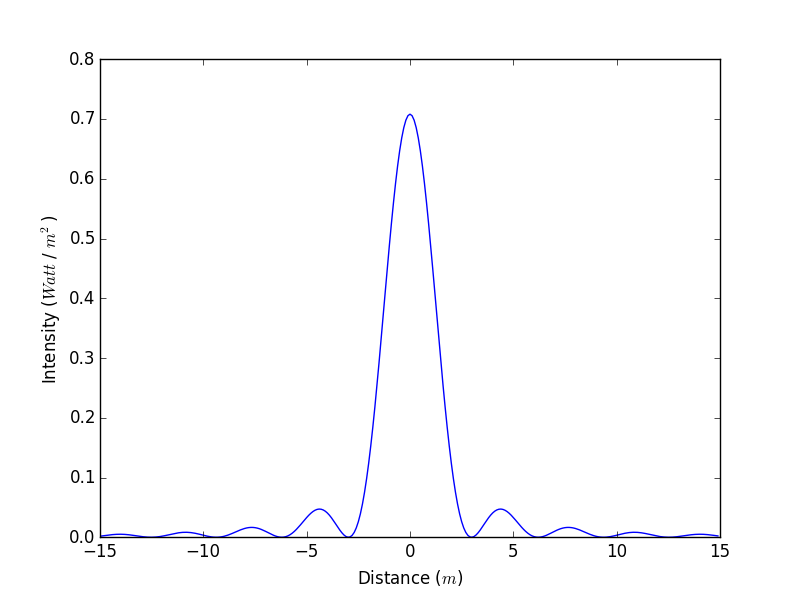
\includegraphics[scale=0.45]{figure_1.png}
\caption{Plot between distance and intensity}
\end{figure}

\begin{flushleft}
	As it should be, Intensity decreases by increasing the distance. Where at the position where source is placed we have high intensity peak.
\end{flushleft}
Next;\\
Plot between distance and intensity, for four antenna sources arrange in a linear array and by managing phase between them, we get interference pattern.
\begin{verbatim}
import numpy as np
import matplotlib.pyplot as plt
from math import sqrt, sin, pi

w=1.0
k=1.0
L=10.0 / k
P=0
# Calculate fringe spacing:
#d = 2 * 5           # Slit-spacing
#fs = 2 * pi * L / (k * d)

#print("Slit-spacing = {} produces fringe spacing = {}".format(d, fs))

ds = [-12, -4, 4, 12]
#sources=[(distance,phase)]
sources = [(-12, 0), (-4,0), (4,0), (12,0)]

def r(x,d):
return sqrt(L**2+(x-d)**2)

def Ex(x,d,p,t):
return ((x-d)/r(x,d)**2)*(sin(k*r(x,d)-w*t+p))

def Ey(x,d,p,t):
return (L/r(x,d)**2)*(sin(k*r(x,d)-w*t+p))

def I(x,sources,t):
Ox=0
Oy=0
for d, p in sources:
Ox+=Ex(x,d,p,t)
Oy+=Ey(x,d,p,t)

return Ox**2+Oy**2

def trapezoidal(f, a, b, n):
h = float(b - a) / n
s = 0.0
s += f(a)/2.0
for i in range(1, n):
s += f(a + i*h)
s += f(b)/2.0
return s * h

xs=[]
ys=[]

for x in np.linspace(-20,20,1000):
y = trapezoidal(lambda t: I(x,sources,t), -pi/w, pi/w, 100) / (2 * pi)

xs.append(x)
ys.append(y)

plt.plot(xs,ys)
plt.show()   
\end{verbatim}
\begin{figure}[ht]
	\centering	
    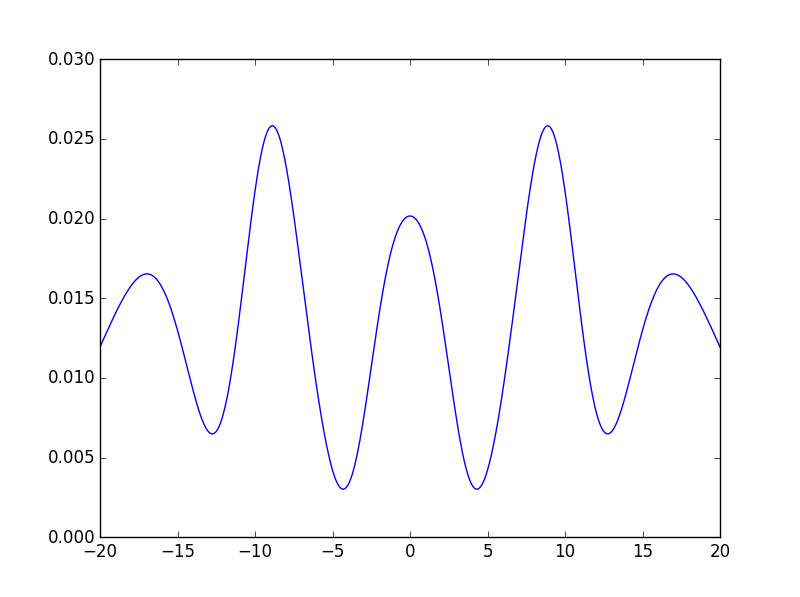
\includegraphics[scale=0.45]{figure_2.png}
	\caption{Plot between distance and intensity}
\end{figure}



%\end{document}
